% =====================================================================
%  Anticythere3D — Manuel d'utilisation / User manual
%  Bilingue FR/EN. Compilation : pdflatex Manuel.tex (deux passes)
% =====================================================================
\documentclass[a4paper,11pt]{article}

\usepackage[utf8]{inputenc}
\usepackage[T1]{fontenc}
\usepackage[french]{babel}
\usepackage{geometry}
\usepackage{graphicx}
\usepackage{xcolor}
\usepackage{colortbl}
\usepackage{tabularx}
\usepackage{booktabs}
\usepackage{array}
\usepackage{amsmath}
\usepackage{tcolorbox}
\usepackage{fancyhdr}
\usepackage{titlesec}
\usepackage{enumitem}
\usepackage{pifont}
\usepackage[hidelinks]{hyperref}

\geometry{left=2.2cm, right=2.2cm, top=2.5cm, bottom=2.3cm}
\DeclareUnicodeCharacter{00B0}{\ifmmode^\circ\else\textdegree\fi}

\definecolor{deepblue}{HTML}{1a3a5c}
\definecolor{accentblue}{HTML}{2980b9}
\definecolor{verylightblue}{HTML}{ebf5fb}
\definecolor{lightblue}{HTML}{d6eaf8}
\definecolor{accentgreen}{HTML}{27ae60}
\definecolor{lightgreen}{HTML}{d5f5e3}
\definecolor{accentorange}{HTML}{e67e22}
\definecolor{lightorange}{HTML}{fdebd0}
\definecolor{accentred}{HTML}{c0392b}
\definecolor{lightred}{HTML}{fadbd8}
\definecolor{darkgray}{HTML}{2c3e50}
\definecolor{medgray}{HTML}{7f8c8d}
\definecolor{lightgray}{HTML}{ecf0f1}
\definecolor{parchment}{HTML}{f5f0e6}

\tcbuselibrary{skins, breakable}
\newtcolorbox{astuce}[1][Astuce]{colback=lightgreen, colframe=accentgreen,
  fonttitle=\bfseries\color{white}, coltitle=white, colbacktitle=accentgreen,
  title={\ding{72}\ \ #1}, arc=3mm, boxrule=0.8pt, left=4mm, right=4mm,
  top=2mm, bottom=2mm, breakable}
\newtcolorbox{info}[1][Pour comprendre]{colback=verylightblue,
  colframe=accentblue, fonttitle=\bfseries\color{white}, coltitle=white,
  colbacktitle=accentblue, title={\ding{42}\ \ #1}, arc=3mm, boxrule=0.8pt,
  left=4mm, right=4mm, top=2mm, bottom=2mm, breakable}
\newtcolorbox{attention}[1][Attention]{colback=lightred, colframe=accentred,
  fonttitle=\bfseries\color{white}, coltitle=white, colbacktitle=accentred,
  title={\ding{68}\ \ #1}, arc=3mm, boxrule=0.8pt, left=4mm, right=4mm,
  top=2mm, bottom=2mm, breakable}
\newtcolorbox{english}[1][English]{colback=lightorange, colframe=accentorange,
  fonttitle=\bfseries\color{white}, coltitle=white, colbacktitle=accentorange,
  title={\ding{110}\ \ #1}, arc=3mm, boxrule=0.8pt, left=4mm, right=4mm,
  top=2mm, bottom=2mm, breakable}

\titleformat{\section}{\Large\bfseries\color{deepblue}}{\thesection.}{0.6em}{}
  [{\color{accentblue}\titlerule[1pt]}]
\titleformat{\subsection}{\large\bfseries\color{accentblue}}{\thesubsection.}{0.5em}{}

\setlength{\headheight}{14pt}
\pagestyle{fancy}
\fancyhf{}
\fancyhead[L]{\small\color{medgray}Anticythere3D — manuel}
\fancyhead[R]{\small\color{medgray}\leftmark}
\fancyfoot[C]{\small\color{medgray}\thepage}
\renewcommand{\headrulewidth}{0.4pt}

\begin{document}

\begin{titlepage}
\centering
\vspace*{2cm}
{\fontsize{30}{34}\selectfont\bfseries\color{deepblue} Anticythere3D}\\[6mm]
{\Large Simulateur de la machine d'Anticythère}\\[2mm]
{\large\color{medgray} Manuel d'utilisation — \textit{User manual}}\\[12mm]
{\color{accentblue}\rule{0.5\textwidth}{1pt}}\\[10mm]
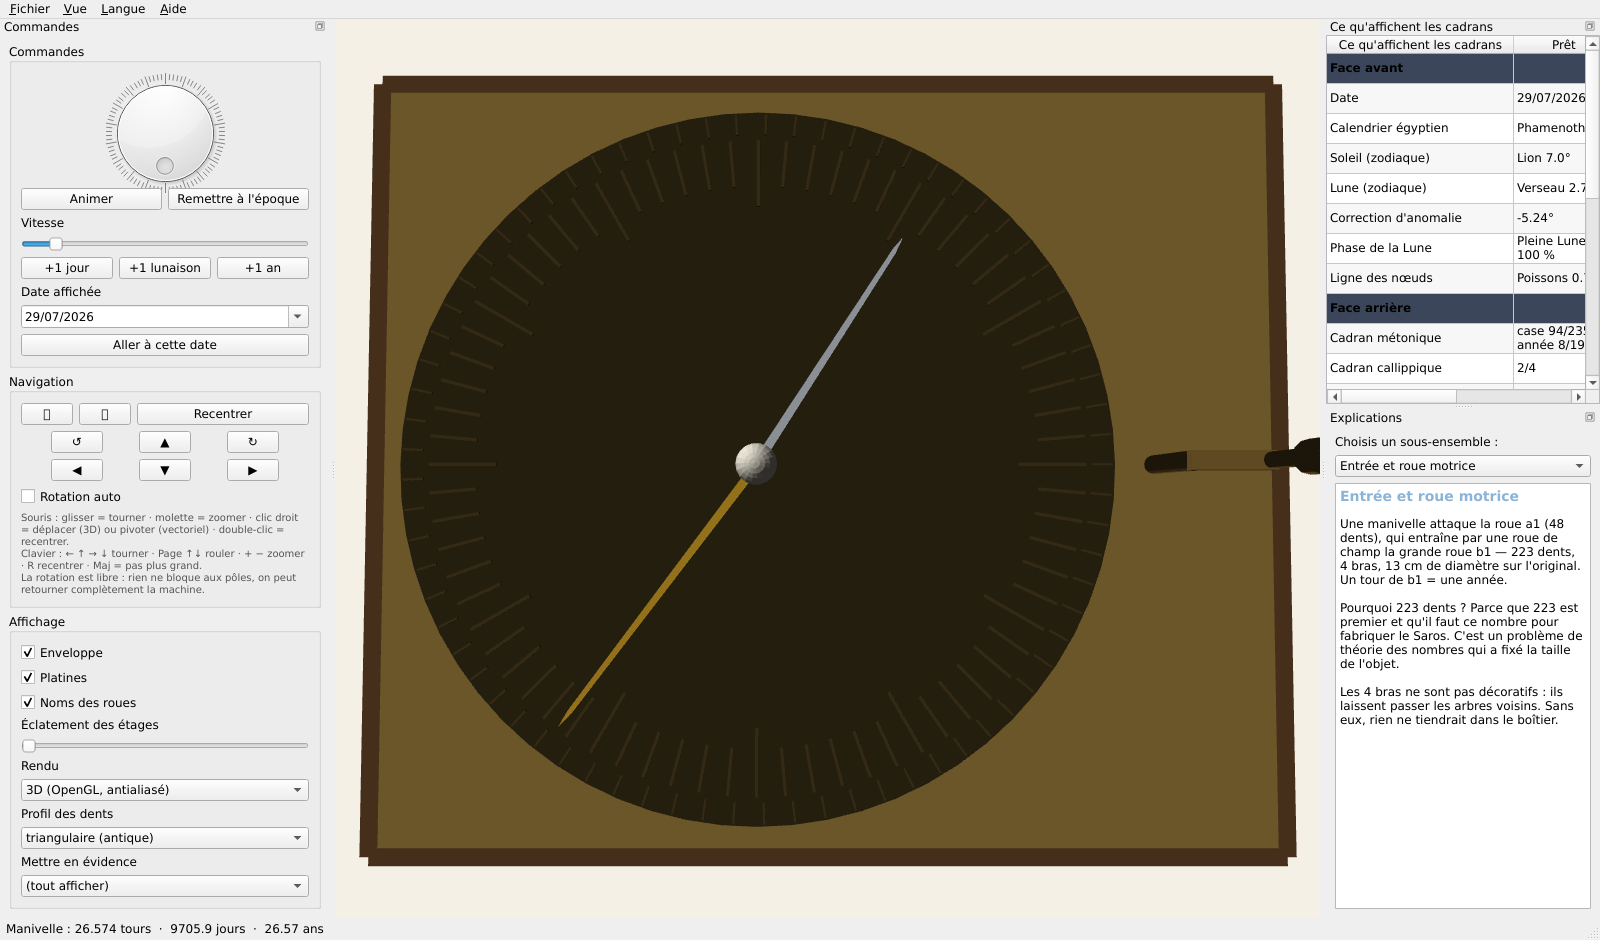
\includegraphics[width=0.86\textwidth]{ferme_avant.png}\\[8mm]
{\large La machine fermée : cadran du zodiaque, aiguilles du Soleil et de la\\
Lune, bille de phase, et la manivelle sur le flanc.}\\[14mm]
{\color{medgray}\small 33 roues \ $\cdot$\ 15 arbres \ $\cdot$\ 2\,231 dents\\
Rapports exacts d'après Freeth \textit{et al.}, \textit{Nature} 2006 \& 2008,
\textit{Scientific Reports} 2021}
\end{titlepage}

\tableofcontents
\newpage

% =====================================================================
\section{Installation}

\subsection{Le programme s'installe tout seul}

Il suffit d'avoir \textbf{Python 3.10 ou plus récent}. Tout le reste — y compris
la 3D — est installé par le programme lui-même au premier démarrage :

\begin{center}
\begin{tcolorbox}[colback=lightgray, colframe=darkgray, width=0.85\textwidth,
  arc=2mm, fontupper=\ttfamily]
python run.py
\end{tcolorbox}
\end{center}

Au premier lancement, le programme détecte ce qui manque, l'annonce, et
l'installe avec \texttt{pip} :

\begin{center}
\begin{tcolorbox}[colback=parchment, colframe=medgray, width=0.9\textwidth,
  arc=2mm, fontupper=\ttfamily\small]
{[}Anticythere3D{]} Dépendances manquantes : PyQt6, numpy, pyqtgraph, OpenGL\\
{[}Anticythere3D{]} Installation automatique en cours…
\end{tcolorbox}
\end{center}

\begin{astuce}[Ce qu'il installe, et où]
Quatre paquets : \texttt{PyQt6} (l'interface), \texttt{numpy} (la géométrie),
\texttt{pyqtgraph} et \texttt{PyOpenGL} (la vue 3D). Hors environnement
virtuel, l'installation se fait avec \texttt{-{}-user} : \textbf{rien n'est
écrit dans les paquets système}. Si tu préfères un environnement isolé :
\begin{center}\ttfamily
python -m venv .venv\\
.venv$\backslash$Scripts$\backslash$activate \ \ (Windows) \ \ ou \ \ source .venv/bin/activate\\
python run.py
\end{center}
\end{astuce}

\subsection{Vérifier sans rien installer}

\begin{center}
\begin{tabularx}{0.95\textwidth}{@{}lX@{}}
\toprule
\rowcolor{lightblue}\textbf{Commande} & \textbf{Effet} \\
\midrule
\texttt{python run.py -{}-check} & liste ce qui manque, n'installe rien, sort \\
\texttt{python run.py -{}-no-install} & démarre sans rien installer \\
\texttt{python run.py -{}-lang en} & interface en anglais \\
\texttt{python run.py -{}-vector} & démarre en rendu vectoriel \\
\texttt{python run.py -{}-samples 16} & antialiasing plus poussé (défaut : 8) \\
\bottomrule
\end{tabularx}
\end{center}

\begin{attention}[Si la 3D ne s'installe pas]
Sur certaines machines sans pilote OpenGL (serveur, machine virtuelle,
bureau à distance), \texttt{pyqtgraph} ou \texttt{PyOpenGL} peuvent
s'installer sans que la 3D fonctionne. \textbf{Le programme ne plante pas} :
il bascule tout seul en \emph{rendu vectoriel}, qui montre les mêmes rotations,
sans aucune dépendance graphique. Rien n'est perdu — au contraire, ce mode
exporte en SVG et en PDF.
\end{attention}

% =====================================================================
\section{Prise en main en deux minutes}

\begin{enumerate}[leftmargin=7mm, itemsep=2mm]
  \item Lance \texttt{python run.py}. La machine apparaît \textbf{fermée},
        comme on la trouverait sur une étagère : coffret de bois, façade de
        bronze gravée, aiguilles, manivelle sur le côté.
  \item Tourne le \textbf{bouton rond} en haut à gauche : c'est la manivelle.
        Un tour complet vaut une année.
  \item Décoche \textbf{Enveloppe} : le coffret disparaît et les 33 roues
        apparaissent, en train de tourner.
  \item Regarde le panneau de droite : il donne en permanence ce que lisait le
        propriétaire de la machine.
\end{enumerate}

\begin{center}
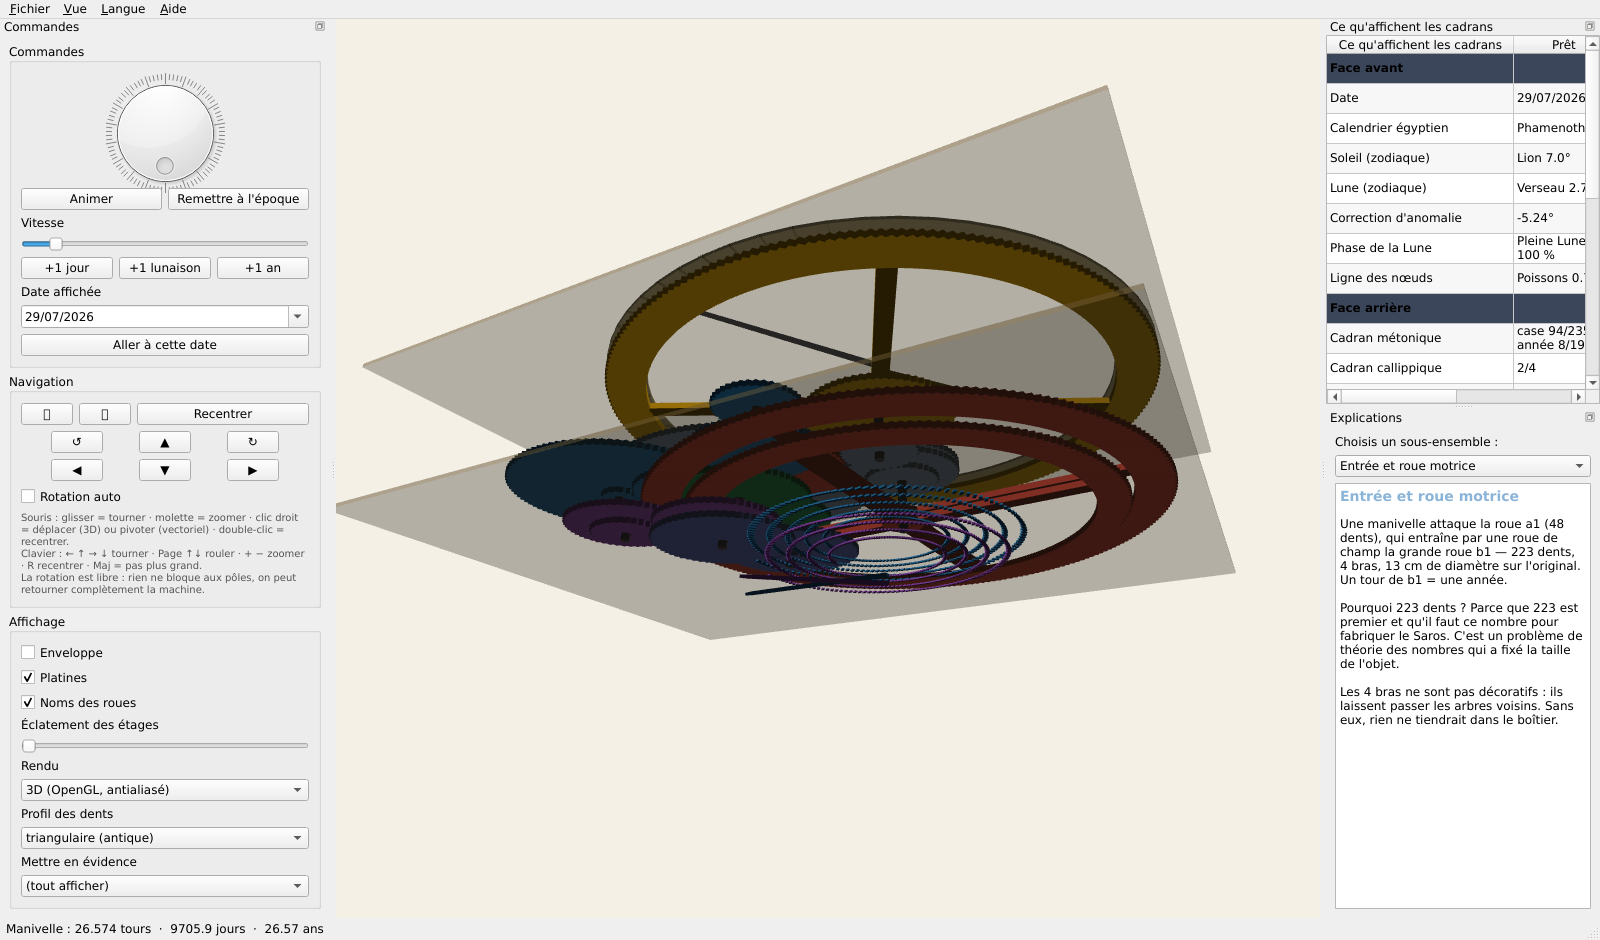
\includegraphics[width=0.92\textwidth]{ouvert_iso.png}\\[2mm]
{\small\color{medgray} L'enveloppe retirée : les 33 roues, les 15 arbres et
les deux grandes roues à bras (b1 devant, e3 derrière).}
\end{center}

% =====================================================================
\section{L'interface}

\subsection{Commandes}

\begin{center}
\begin{tabularx}{\textwidth}{@{}lX@{}}
\toprule
\rowcolor{lightblue}\textbf{Élément} & \textbf{Rôle} \\
\midrule
Bouton rond & la manivelle : la \textbf{seule} entrée de la machine \\
Animer / Pause & fait tourner la manivelle en continu \\
Vitesse & nombre de jours simulés par seconde \\
+1 jour / +1 lunaison / +1 an & avance d'un pas exact \\
Remettre à l'époque & ramène la machine à sa date de calage \\
Date affichée + Aller à cette date & saute directement à une date \\
\bottomrule
\end{tabularx}
\end{center}

\begin{info}[Pourquoi une seule entrée ?]
Parce que la machine réelle n'en a qu'une. Tout le reste — Soleil, Lune,
phase, éclipses, calendriers — n'est pas « calculé » séparément : ce sont des
rapports d'engrenages, donc des conséquences mécaniques du seul mouvement de
la manivelle. C'est exactement ce que fait le programme : il n'y a aucune
formule d'affichage, seulement des fractions de nombres de dents.
\end{info}

\subsection{Navigation : zoomer, tourner, retourner}

\begin{center}
\begin{tabularx}{\textwidth}{@{}p{5.2cm}X@{}}
\toprule
\rowcolor{lightblue}\textbf{Geste} & \textbf{Effet} \\
\midrule
Glisser à la souris & faire tourner l'objet \\
Molette & zoomer / dézoomer \\
Clic droit et glisser & déplacer (3D) ou pivoter (vectoriel) \\
Double-clic & recentrer \\
$\leftarrow\ \uparrow\ \rightarrow\ \downarrow$ & tourner au clavier \\
Page $\uparrow$ / Page $\downarrow$ & rouler (3\textsuperscript{e} axe) \\
\texttt{+} / \texttt{-} & zoomer / dézoomer \\
\texttt{R} & recentrer \\
\texttt{Maj} enfoncée & pas de rotation plus grand \\
\texttt{Espace} & animer / pause \\
\texttt{F} / \texttt{B} / \texttt{I} & face avant / arrière / vue 3/4 \\
\bottomrule
\end{tabularx}
\end{center}

\begin{astuce}[Rotation vraiment libre]
La caméra est pilotée par \emph{quaternion} et non par angles d'Euler :
\textbf{rien ne bloque aux pôles}. On peut passer au-dessus, continuer, et
retourner complètement la machine — ce qui est impossible dans la plupart des
visionneuses 3D, qui butent à 90° d'élévation.
\end{astuce}

\subsection{Affichage}

\begin{center}
\begin{tabularx}{\textwidth}{@{}lX@{}}
\toprule
\rowcolor{lightblue}\textbf{Réglage} & \textbf{Effet} \\
\midrule
\textbf{Enveloppe} & montre ou retire le coffret, la façade et la manivelle \\
Platines & les deux plaques intérieures qui portent les arbres \\
Noms des roues & étiquette chaque roue avec son nombre de dents \\
Éclatement des étages & écarte les 16 plans d'engrènement \\
\textbf{Rendu} & 3D temps réel, ou vectoriel exportable \\
\textbf{Profil des dents} & triangulaire (antique) ou développante (moderne) \\
Mettre en évidence & n'éclaire qu'un sous-ensemble, éteint les autres \\
\bottomrule
\end{tabularx}
\end{center}

\begin{info}[Les deux profils de dents]
Les dents de la machine réelle sont des \textbf{triangles quasi équilatéraux}.
Le rapport \emph{moyen} est alors rigoureusement exact — c'est pour cela que
l'instrument est juste — mais le rapport \emph{instantané} oscille à chaque
passage de dent. La \textbf{développante de cercle}, inconnue des Grecs, est le
seul profil qui donne un rapport constant à tout instant. Basculer entre les
deux dans le programme montre la différence de forme.
\end{info}

\subsection{Le rendu vectoriel}

\begin{center}
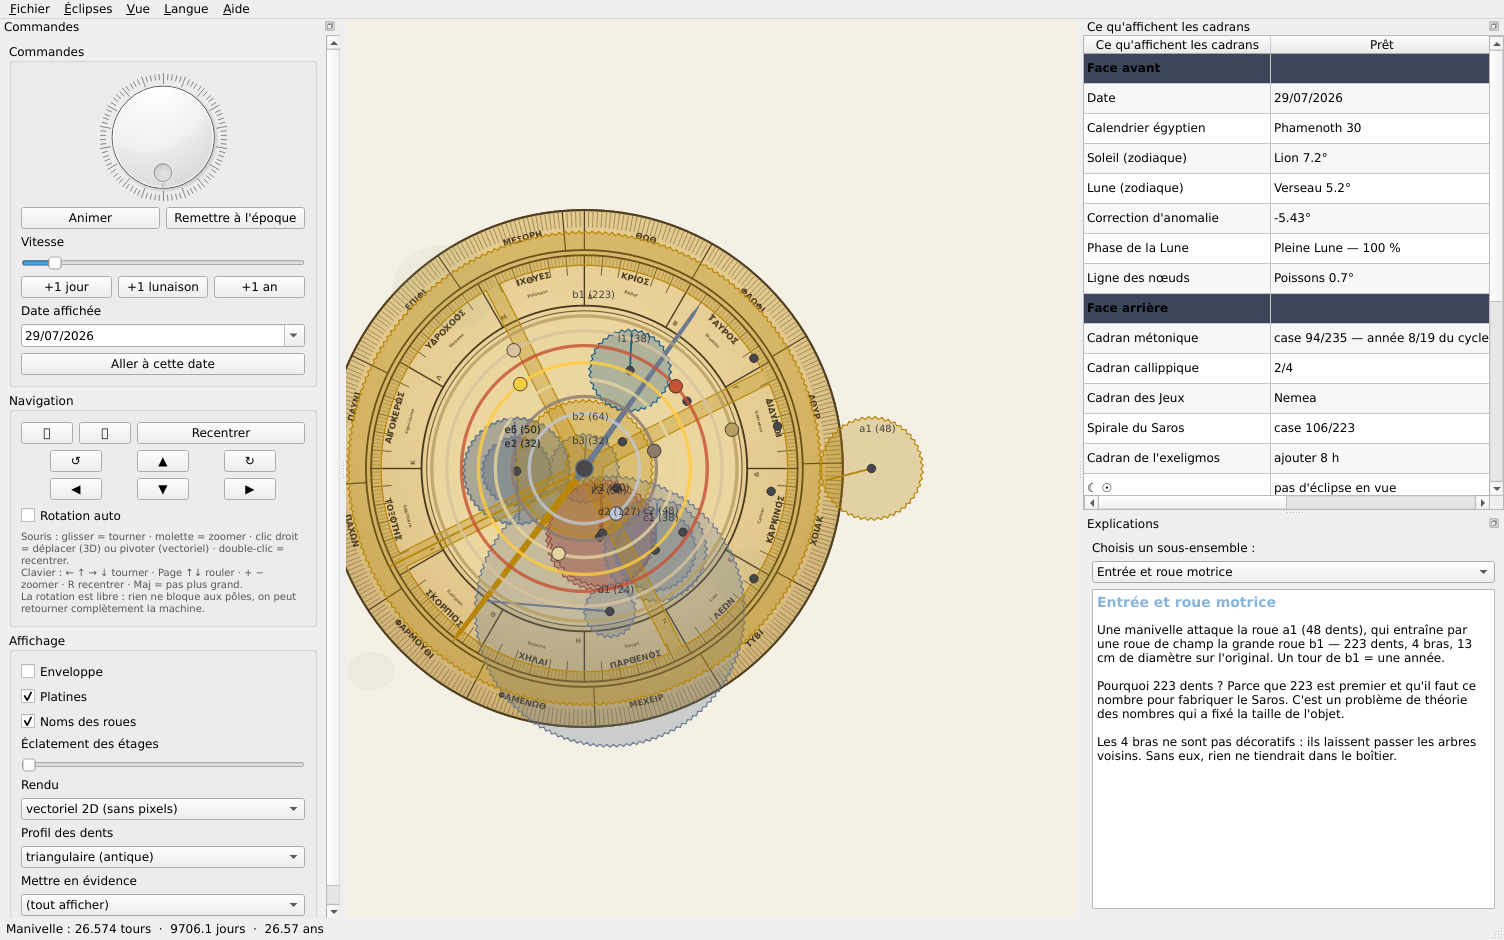
\includegraphics[width=0.92\textwidth]{vue_vectorielle.png}\\[2mm]
{\small\color{medgray} Rendu vectoriel : chaque dent est une courbe, pas un
pixel. Zoom, déplacement, et export sans perte.}
\end{center}

Ce mode dessine les \textbf{dentures réelles} en courbes. Il sert à trois
choses :
\begin{itemize}[leftmargin=6mm]
  \item regarder le mécanisme à plat, sans occlusion ;
  \item exporter en \textbf{SVG} ou en \textbf{PDF A3} — les fichiers ne
        contiennent aucune image bitmap, on peut donc imprimer en A0 ou zoomer
        indéfiniment sans voir un seul pixel ;
  \item fonctionner sur une machine dépourvue d'OpenGL.
\end{itemize}

% =====================================================================
\newpage
\section{Ce qu'affichent les cadrans}

\subsection{Le panneau de report}

Le panneau de droite se détache (c'est une fenêtre à part entière) et donne :

\begin{center}
\small
\begin{tabularx}{\textwidth}{@{}lX@{}}
\toprule
\rowcolor{lightblue}\textbf{Ligne} & \textbf{Signification} \\
\midrule
Date & date grégorienne correspondant à la position de la manivelle \\
Calendrier égyptien & mois et jour du calendrier de 365 jours de la face avant \\
Soleil (zodiaque) & position du Soleil moyen — c'est aussi le pointeur de date \\
Lune (zodiaque) & position de la Lune, anomalie comprise \\
Correction d'anomalie & écart produit par le tenon-fente, au plus $\pm 6{,}58°$ \\
Phase de la Lune & nom de la phase et pourcentage éclairé \\
Ligne des n\oe uds & position des n\oe uds, qui décide des éclipses \\
Cadran métonique & case sur 235 et année sur 19 du cycle \\
Cadran callippique & quart sur 4 du cycle de 76 ans \\
Cadran des Jeux & jeu panhellénique de l'année \\
Spirale du Saros & case sur 223 \\
Cadran de l'exeligmos & correction horaire à ajouter : 0, 8 ou 16 heures \\
\textbf{Lune et Soleil} & annonce d'éclipse possible ou quasi certaine \\
Planètes & positions selon le modèle de Freeth \textit{et al.} (2021) \\
Écart machine / ciel réel & \textbf{l'erreur de l'instrument}, en degrés \\
\bottomrule
\end{tabularx}
\end{center}

\begin{info}[La dernière ligne est la plus intéressante]
Le programme compare en permanence ce qu'affiche la machine à ce que donnent
les éphémérides modernes. Sur le Soleil moyen, l'écart est \textbf{nul} : le
rapport est exactement 1. Sur la Lune, il atteint quelques degrés par siècle,
et ce n'est pas un défaut du logiciel — c'est l'erreur réelle de l'instrument.
Elle se décompose ainsi :
\[
\underbrace{2{,}2°}_{\substack{\text{évection et variation}\\ \text{non mécanisées}}}
\;+\;
\underbrace{3{,}5°\ \text{par 50 ans}}_{\substack{\text{dérive de}\\ 254/19}}
\;+\;
\underbrace{0{,}8°}_{\substack{\text{précession de}\\ \text{l'apogée}}}
\]
La suite de tests du programme vérifie que l'erreur mesurée reste sous ce
budget : c'est une manière de prouver que le simulateur est fidèle \emph{y
compris dans ses défauts}.
\end{info}

\subsection{Lire les gravures}

Les cadrans eux-mêmes portent des inscriptions, reproduites d'après les
fragments. Retourne la machine (bouton \textsf{Arrière}) et zoome : tout est
gravé, en vectoriel, donc net à n'importe quel grossissement.

\begin{center}
\small
\begin{tabularx}{\textwidth}{@{}llX@{}}
\toprule
\rowcolor{lightblue}\textbf{Cadran} & \textbf{Divisions} & \textbf{Ce qui est écrit} \\
\midrule
\multicolumn{3}{@{}l}{\textit{Face avant}}\\
Zodiaque & $12 \times 30°$ & les douze signes en grec depuis le point vernal ;
noter \emph{Ch\^elai}, «~les pinces~», là où nous disons Balance \\
Parapegma & lettres & petites lettres-index semées dans le zodiaque, renvoyant
à un calendrier d'étoiles gravé sur la plaque \\
Calendrier & 365 ou 354 & les mois égyptiens en caractères grecs ; l'anneau est
\textbf{mobile}, on le tourne d'un cran tous les quatre ans \\
\midrule
\multicolumn{3}{@{}l}{\textit{Face arrière}}\\
Métonique & spirale, 235 cases & une case = un mois lunaire, avec le nom de son
mois corinthien sur le tour extérieur ; le numéro d'année en chiffres grecs
marque chacune des 19 années \\
Callippique & 4 secteurs & lequel des quatre cycles de 76 ans on parcourt \\
Jeux & 4 secteurs & \emph{Olympia}, \emph{Nemea}, \emph{Isthmia},
\emph{Pythia} — le seul cadran non astronomique \\
Saros & spirale, 223 cases & les cases où une éclipse est possible portent
$\mathrm{H}$ (\^eta, pour \emph{H\^elios}, le Soleil) ou $\Sigma$ (sigma, pour
\emph{Sel\^en\^e}, la Lune) \\
Exeligmos & 3 secteurs & 0, 8 ou 16 heures à \textbf{ajouter} à l'heure lue
sur le Saros \\
\bottomrule
\end{tabularx}
\end{center}

\begin{info}[Les sept années à treize mois]
Dix-neuf années solaires valent 235 mois lunaires, or $19 \times 12 = 228$ :
sept années du cycle en comptent \textbf{treize}. Elles se répartissent selon
le critère $(12k) \bmod 19 < 7$, soit les années $2, 5, 8, 10, 13, 16, 19$ —
et le total retombe sur 235 cases exactement. C'est pourquoi les traits de
début d'année ne sont pas régulièrement espacés sur la spirale.
\end{info}

\begin{info}[Pourquoi 223 cases sur le Saros]
Parce que trois périodes lunaires y coïncident à moins de cinq heures près sur
dix-huit ans : 223 mois synodiques (même phase), 242 draconitiques (même
n\oe ud), 239 anomalistiques (même distance). L'éclipse se répète. Il reste
$0{,}321$ jour, qui la décale de $7{,}7$~heures — environ $116°$ de longitude,
donc souvent invisible de chez soi. Après trois Saros, ce reste fait presque un
jour entier : c'est ce que compte le cadran de l'exeligmos.

\textbf{Réserve} : les glyphes d'éclipse sont \textbf{calculés}, pas copiés. Le
motif de la plaque n'est connu que par fragments ; le programme applique le
critère que la machine mécanise — syzygie proche d'un n\oe ud — sur les 223
mois d'un Saros, et marque 48 cases solaires, 32 lunaires, dont 22 portent les
deux. Un peu plus que les glyphes gravés, les limites retenues incluant des
éclipses rasantes.
\end{info}

% =====================================================================
\section{Les rapports, et pourquoi ils sont exacts}

Le menu \textsc{Aide $\rightarrow$ Les mathématiques de la machine} donne la
table complète. Les rapports sont tenus en \textbf{fractions exactes}, jamais
en nombres à virgule :

\begin{center}
\begin{tabularx}{\textwidth}{@{}llX@{}}
\toprule
\rowcolor{lightblue}\textbf{Sortie} & \textbf{Rapport} & \textbf{Contrôle} \\
\midrule
Lune sidérale & $254/19$ & mois sidéral de 27,321\,266 j \\
Porte-satellite $e_3$ & $477/4237$ & 8,8826 ans (apogée réel : 8,8504) \\
Anomalie & — & période de \textbf{27,5533 j} contre 27,554\,55 : \textbf{1,8 minute} \\
Métonique & $5/19$ & 5 tours en 19 ans \\
Callippique & $1/76$ & 1 tour en 76 ans \\
Saros & $940/4237$ & 4 tours pour 223 lunaisons \\
Exeligmos & $235/12711$ & 1 tour en 54,09 ans, soit 3 Saros \\
\bottomrule
\end{tabularx}
\end{center}

\begin{info}[Le mois anomalistique n'est écrit nulle part]
Le tenon et la fente sont montés sur la roue $e_3$, qui tourne en 8,88 ans —
la précession de l'apogée lunaire. La modulation a donc pour période la
\emph{différence} des deux rotations :
\[
  \frac{254}{19} - \frac{477}{4237} = \frac{56\,165}{4237}\ \text{tour/an}
  \quad\Longrightarrow\quad T = 27{,}553\ \text{jours},
\]
à comparer au mois anomalistique réel de 27,554\,55 jours : \textbf{1,8 minute
d'écart}. Ce nombre n'apparaît dans aucune roue : il émerge d'une soustraction
de fréquences réalisée en bronze.
\end{info}

% =====================================================================
\section{Dépannage}

\begin{center}
\begin{tabularx}{\textwidth}{@{}p{5.4cm}X@{}}
\toprule
\rowcolor{lightblue}\textbf{Symptôme} & \textbf{Que faire} \\
\midrule
« Dépendances manquantes » & lancer \texttt{python run.py} une seconde fois,
ou \texttt{pip install -r requirements.txt} \\
Fenêtre noire, pas de 3D & OpenGL indisponible : passer en \textbf{rendu
vectoriel} (le programme le fait tout seul) \\
Dents crénelées & augmenter l'antialiasing : \texttt{-{}-samples 16}, ou passer
en vectoriel \\
Trop lent en animation & baisser la vitesse, décocher \textbf{Noms des roues},
ou revenir en 3D \\
On ne voit que les grandes roues & normal : b1 et e3 recouvrent les petites.
Utiliser \textbf{Éclatement} ou \textbf{Mettre en évidence} \\
Le pointeur ne revient pas pile & vérifier avec les tests :
\texttt{python tests/test\_mechanism.py} \\
\bottomrule
\end{tabularx}
\end{center}

% =====================================================================
\section{Ce qui est fidèle, et ce qui ne l'est pas}

\begin{astuce}[Fidèle et vérifié]
Les 30 roues attestées et leurs nombres de dents, les rapports de tous les
trains, le dispositif à tenon et fente et son porte-satellite, les cadrans
arrière (spirale métonique de 5 tours et 235 cases, spirale du Saros de 4 tours
et 223 cases), le principe de la manivelle unique, les quatre bras de $b_1$.
\end{astuce}

\begin{attention}[Reconstitué ou simplifié]
\begin{itemize}[leftmargin=6mm]
  \item Les \textbf{planètes} sont calculées d'après le modèle de 2021, mais
        pas modélisées en 3D : ce sont des reconstitutions, pas des relevés.
  \item L'\textbf{implantation des arbres} est calculée par optimisation sous
        contraintes ; elle respecte les 17 entraxes exacts, mais ce n'est pas
        la disposition de l'original, qui reste partiellement inconnue.
  \item Les \textbf{gravures} des cadrans (noms de mois, glyphes d'éclipses)
        ne sont pas dessinées ; la prédiction d'éclipse, elle, est calculée.
  \item Le \textbf{boîtier} suit les proportions du mécanisme reconstitué, non
        les 34 $\times$ 18 $\times$ 9 cm de l'original.
\end{itemize}
\end{attention}

% =====================================================================
\newpage
\section*{English — quick guide}
\addcontentsline{toc}{section}{English — quick guide}

\begin{english}[Installation]
You only need \textbf{Python 3.10+}. Run \texttt{python run.py}: the program
detects what is missing and installs it itself, \textbf{3D included}
(PyQt6, numpy, pyqtgraph, PyOpenGL). Outside a virtual environment it installs
with \texttt{-{}-user}, so nothing is written into system packages.
Use \texttt{-{}-check} to inspect without installing, \texttt{-{}-no-install}
to skip it, \texttt{-{}-lang en} for the English interface.
\end{english}

\begin{english}[Getting started]
The machine starts \textbf{closed}: wooden case, engraved bronze front, Sun and
Moon hands, phase ball, side crank. Turn the round knob — one full turn is one
year. Untick \textbf{Case} to remove the housing and watch all 33 gears turn.
\end{english}

\begin{english}[Navigation]
Drag to rotate, wheel to zoom, right-drag to pan (3D) or roll (vector),
double-click to reset. Keyboard: arrows rotate, Page $\uparrow\downarrow$ roll,
\texttt{+}/\texttt{-} zoom, \texttt{R} reset, \texttt{Space} animate,
\texttt{F}/\texttt{B}/\texttt{I} front/back/isometric. The camera uses
quaternions: \textbf{rotation is unconstrained}, nothing locks at the poles,
and the machine can be turned completely upside down.
\end{english}

\begin{english}[Vector mode]
A second rendering mode draws the real tooth outlines as curves and exports to
\textbf{SVG} and \textbf{A3 PDF} with no bitmap inside — print at A0, zoom
forever, no pixels. It is also the automatic fallback when OpenGL is missing.
\end{english}

\begin{english}[Accuracy]
Gear ratios are exact rationals taken from the tomography-derived tooth counts.
The pin-and-slot device, riding on a carrier that turns once per 8.8826 years,
yields a modulation of period \textbf{27.5533 days} — the anomalistic month to
within \textbf{1.8 minutes}. The right-hand panel continuously reports the
mechanism's own error against modern ephemerides.
\end{english}

\vfill
\begin{center}
\begin{tcolorbox}[colback=lightgray, colframe=darkgray, width=0.95\textwidth,
  arc=2mm]
\small
\textbf{Sources.} Freeth T. \textit{et al.}, \textit{Nature} \textbf{444}
(2006) 587–591 ; Freeth T., Jones A., Steele J., Bitsakis Y.,
\textit{Nature} \textbf{454} (2008) 614–617 ; Freeth T., Higgon D.,
Dacanalis A., MacDonald L., Georgakopoulou M., Wojcik A.,
\textit{Scientific Reports} \textbf{11}:5821 (2021) ; Meeus J.,
\textit{Astronomical Algorithms}, 2\textsuperscript{e} éd.
\end{tcolorbox}
\end{center}

\end{document}
